\documentclass{article}
\usepackage[utf8]{inputenc}
\usepackage{amsmath}
\usepackage{amsthm}
\usepackage{amsfonts}
\usepackage{amssymb}
\usepackage{amstext}
\usepackage{gensymb}
\usepackage{graphicx}
\usepackage{enumerate}
\pagenumbering{arabic}
\usepackage{fancyhdr}
\usepackage[margin=0.75in]{geometry}
\usepackage{eucal}
\usepackage{parskip} % removes auto indentation for paragraphs
\usepackage{enumitem} % changes the indexing for enumerate
\setlist[enumerate,1]{label = {(\alph*)}}

\usepackage{mathtools} % used for making a ceiling function

\DeclarePairedDelimiter{\ceil}{\lceil}{\rceil} %create ceiling function as \ceil{x}, \ceil*{x} to add \left and \right

\usepackage{listings} % import code into latex

\usepackage{algorithm} % used to write algorithms
\usepackage[noend]{algpseudocode}

\def\N{\mathbb{N}}
\def\Z{\mathbb{Z}}
\def\Q{\mathbb{Q}}
\def\R{\mathbb{R}}
\newcommand{\Mod}[1]{\ (\text{mod}\ #1)}
\newcommand{\Problem}[1]{\textbf{\large Problem #1}}
\newcommand{\li}[0]{\liminf_{n\to\infty}}
\newcommand{\ls}[0]{\limsup_{n\to\infty}}
\newcommand{\dl}[2]{\displaystyle\lim_{#1 \to #2}}
\newcommand{\ds}[2]{\displaystyle\sum_{#1}^{#2}}
\newcommand{\ra}{\Rightarrow}

\linespread{1.5}

\usepackage{float}

\title{CSE 6140 - Homework 3}
\author{Alexander Winkles}
\date{}


\begin{document}

\maketitle

\vspace{2in}



\newpage

\Problem{1}

To prove this problem, which we will call $FIBER$, is NP-Complete we will first show $FIBER \in \mathcal{NP}$, then we will show for some already known NP-Complete problem $Y$ that $Y \leq_p FIBER$. 

\newtheorem{np}{Theorem}
\begin{np}
$FIBER \in \mathcal{NP}$.
\end{np}
\begin{proof} % fix certificate
To show this, we must find a certificate $T$ and a certifier $B$ that runs in polynomial time. 
Let $T$ be a subset of $C$.
The certifier will then check that all cities are connected using the roads within $T$ and that for each $t \in T$, that $1 \leq d_T(t) \leq k$. 
Both of these can be done in polynomial time, which completes the proof. 
\end{proof}

\begin{np}
$FIBER$ is NP-Complete. 	
\end{np}
\begin{proof}

Consider an arbitrary instance of the Hamiltonian Path problem with $k'$ vertices. 
Our goal is to transform this instance into a single instance of $FIBER$ with identical solutions.
For each node in $HAM-PATH$, we make a city $c \in C$ for $FIBER$.
From this, add the corresponding edges such that $k = 2$ for $FIBER$. 
With this construction, we will prove that the two problems have corresponding solutions.

First, consider some instance of $HAM-PATH$.
By construction, every node in $HAM-PATH$ becomes a city in $FIBER$, and as $HAM-PATH$ is connected it follows that every city is present in $FIBER$. 
Additionally, by construction the connecting path of $HAM-PATH$ are the roads in $FIBER$, so all the cities are connected with $d_T(u) \leq 2\ \forall u \in C$. 
Thus when $HAM-PATH$ is solved so too is $FIBER$.

Now consider an instance of $FIBER$ with $k = 2$. 
For each city in the instance, we have a node for a graph.
Additionally, for each road in $FIBER$ we will have an edge between nodes in the graph. 
Since the cities in $FIBER$ are connected, so too must all the nodes be in the graph by construction.
Likewise, since $k = 2$ for $FIBER$, the resulting edges must create a path.
Thus when $FIBER$ is solved so too is $HAM-PATH$. 

Thus, $HAM-PATH\leq_p FIBER$ and $FIBER$ is NP-Complete. 
\end{proof}

\Problem{2}

To show that $PYGMALION$ is NP-Complete, we will first show that $PYGMALION \in \mathcal{NP}$. 
\begin{np}
$PYGMALION \in \mathcal{NP}$. 	
\end{np}
\begin{proof}
To show this, we must find a certificate $T$ and a certifier $B$ that runs in polynomial time.
Let $T$ be a subset of towns where the bunkers will be placed. 
The certifier will then check that there are at most $k$ bunkers (i.e. $|T| \leq k$) and that each $e = (u,v) \in E$ satisfies $u \in T$ or $v \in T$. 
Both of these can be done in polynomial time by simply counting the cardinality of $T$ and checking if a node is in $T$, so the proof is complete. 
\end{proof}
\begin{np}
$PYGMALION$ is NP-Complete. 	
\end{np}
\begin{proof}
Consider an arbitrary instance of the Vertex Cover problem.
Our goal is to transform this instance into a single instance of $PYGMALION$ with identical solutions.
For an instance of $VC$, anytime there is a node of degree 2 or more, duplicate it and make both the original node and its new copy into towns for $PYGMALION$. 
Turn each original edge into a road, then add an additional road connecting the original node to its duplicate. 
Additionally add roads that connect the duplicate node to all the nodes connected to the original node. 
With this construction, we will prove that the two problems have corresponding solutions.

Consider some instance of $VC$ that is solved. 
That means we have some set $T \subseteq V$ that touch every edge in $E$. 
If any of the duplicated nodes in $PYGMALION$ were nodes in $T$, we can pick either the newly created town or the original town to place a bunker on; otherwise we pick the same town to place a bunker on corresponding to the node in $T$. 
By our construction, since we duplicate any node of of degree 2 or more then add corresponding edges, all of the towns with bunkers will cover all of the towns not connected by bunkers, so when $VC$ is solved so too is $PYGMALION$.

Consider some instance of $PYGMALION$ that is solved.
Thus we have bunkers placed at towns in such a way that every town in either connected to a bunker or has a bunker. 
If there are two towns that have identical roads and are themselves connected, we can consolidate them by ``deconstruction''. 
Because every town is adjacent to or on a bunker, all roads are connected to a bunker.
This is by definition a vertex cover, so we are done.

Thus, $VC \leq_p PYGMALION$ and the proof is complete. 

\end{proof}

\Problem{3}

For this problem, I wrote both a divide \& conquer algorithm and a dynamic programming algorithm to find the maximum sum subset of given files. 
Below is the graph comparing the two methods:
\begin{figure}[H]
\centering
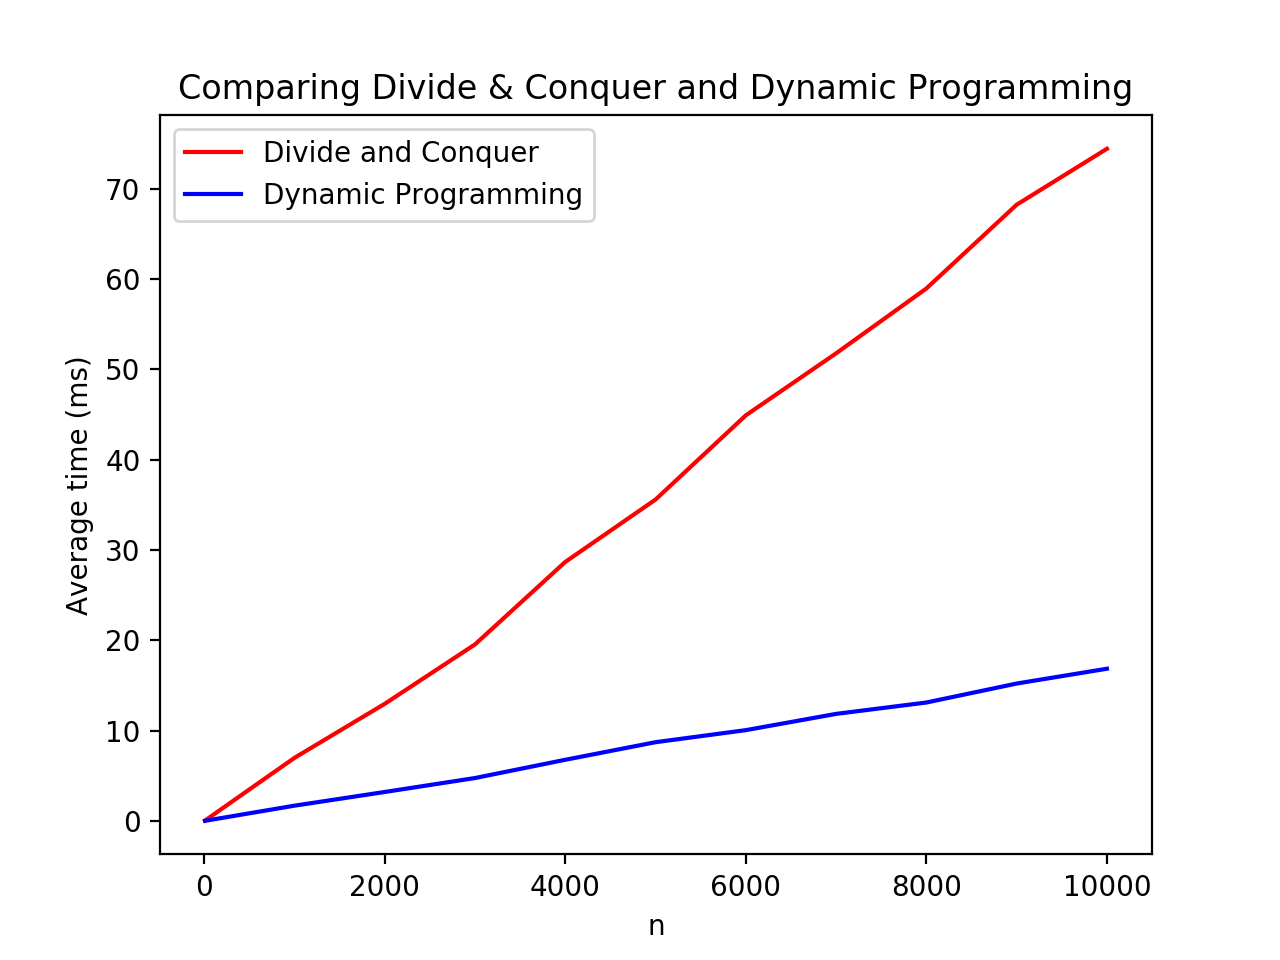
\includegraphics[height=7cm]{comparison}
\end{figure}


My divide \& conquer algorithm was designed as follows.
It takes in an array of values, a start index, and a start index.
If the start index equals the stop, the algorithm returns the value of the array at said index.
Otherwise it computes the midpoint of the two indices (rounding down) then recursively calls two instances of itself for the intervals (start, mid) and (mid + 1, stop).
Additionally, a cross method is called that computes the largest sum within the middle of the set. 
Of these values, the maximum is returned along with the corresponding indices. 
The space complexity of this program is $O(n)$, as there are several variables and an array of size $n$. 
The time complexity can be expressed by the recurrence relationship $T(n) = 2T(n/2) + \Theta(n)$, which by the Master theorem gives us complexity of $\Theta(n\log{n})$. 
This can be seen in the above figure, which matches this complexity well. 

My dynamic programming algorithm was designed as follows.
It takes in an array of values, then creates two arrays of size $n$. 
A for loop is then run that computes the following recurrence relation:
\begin{equation*}
B(j) = 
\begin{cases}
	0 \qquad\qquad\qquad\qquad\qquad\quad\ \, j = 0\\
	\max{\{B(j-1) + a_j, 0\}}\qquad \text{otherwise}\\
\end{cases}	
\end{equation*}
It additionally computes the corresponding indices that give $B(n)$. 
The space complexity of tis program is $O(n^3)$, as there is the initial values array, then two arrays of same size are create to store $B(j)$ values and start indices. 
The time complexity is $O(n)$ as there is a single for loop that calls on precomputed values from an array. 
This complexity can be seen in the above figure. 

By the above analysis, the dynamic programming algorithm should be faster than the divide \& conquer one by a significant amount for large $n$. 
This can be seen in the graph above, with the dynamic programming one consistently outperforming the divide \& conquer. 
Note that this comes as a trade off - if $n$ becomes incredible large far more memory must be committed for DP, which could potentially change the results of the analysis. 


\end{document}